\subsection{Масштабирование}
В облачных решениях захват всех аппаратных ресурсов невозможен вследствие ограниченного выделения ресурсов каждой из задач~\cite{fake-23}.
В общем случае, это способы ограничения ресурсов делятся на два типа~\cite{containers-and-vm-big-data}:
\begin{itemize}
    \item решения на базе виртуальных машин;
    \item решения на базе контейнеров.
\end{itemize}

В обоих подходах количество ресурсов, доступных задаче, управляются с помощью масштабирования. Различают два типа масштабирования.
\begin{enumerate}
    \item Горизонтальное.
    
    Горизонтальным называется масштабирование, при котором изменяется количество виртуальных машин или контейнеров, доступных задаче.
    Количество ресурсов, доступных каждой из виртуальных машин или каждому из контейнеров, при этом остаётся неизменным.
    \item Вертикальное.
    
    Вертикальным масштабированием называется такое масштабирование, при котором изменяется количество ресурсов, выделенных каждой из виртуальных машин или контейнеров.
    Их количество при этом остаётся неизменным.
\end{enumerate}
Разница между ними проиллюстрирована на рис.~\ref{scale-out-up}.

\begin{figure}[H]
    \centering
    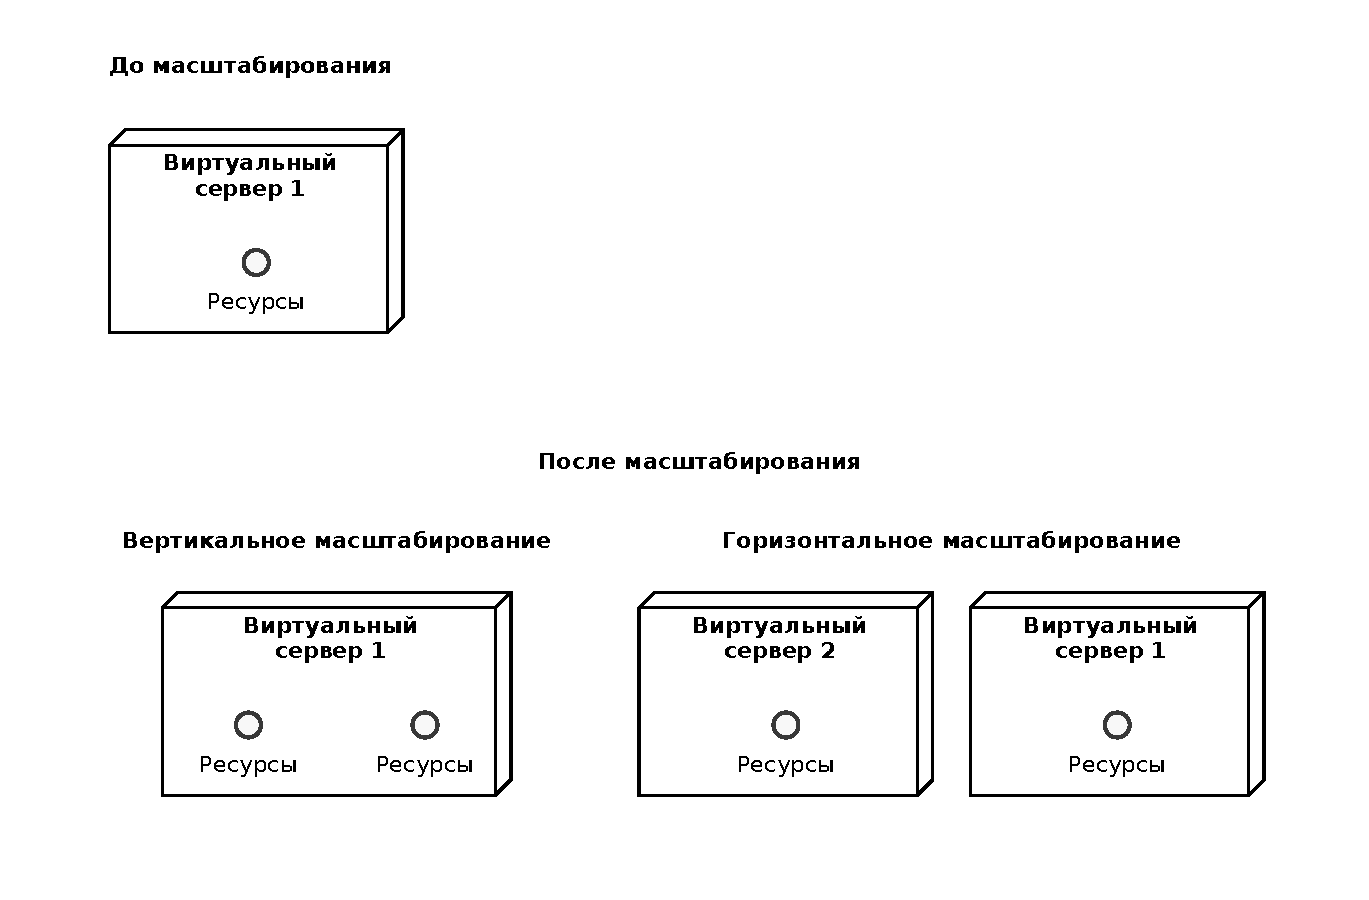
\includegraphics[width=\textwidth]{img/scale-out-up.pdf}
    \caption{Сравнение горизонтального и вертикального масштабирования}
    \label{scale-out-up}
\end{figure}

Горизонтальное масштабирование в настоящее время применяется чаще~\cite{fake-24} по ряду причин, неполный перечень которых представлен далее.
\begin{enumerate}
    \item Возможность выделения на одно приложение (задачу) несколько серверов.
    
    Это достигается при помощи запуска виртуальных машин или контейнеров на каждом из из серверов~\cite{fake-28}.
    
    \item Более высокая загрузка аппаратного обеспечения.
    
    В случае отсутствия нагрузки на приложение, будет простаивать только то количество аппаратных ресурсов, которое выделено одной виртуальной машине или контейнеру приложения, другие ресурсы при этом будут высвобождены~\cite{fake-25}.
    В случае горизонтального масштабирования есть возможность выделить одной виртуальной машине или контейнеру минимально необходимое количество ресурсов для обработки минимальной нагрузки на приложение
    В то же время в случае вертикального масштабирования, при выделении ресурсов, достаточных для обработки пиковой нагрузки, будет наблюдаться простой в обычном режиме работы~\cite{fake-26}. 
\end{enumerate}

Таким образом, существует задача масштабирования приложений.
Для решения этой задачи существуют технологии, имеющие общее название ''автомасштабирование''~\cite{portable-autoscaler-for-managing-multi-cloud-elasticity}.
При помощи таких технологий осуществляется автоматическое масштабирование в зависимости от текущей нагрузки на приложение или других факторов.

Во многие платформы облачных вычислений сервисы автомасштабирования уже встроены~\cite{fake-32}, однако существуют сервисы автомасштабирования, являющиеся внешними по отношению к платформе, как показано на рис.~\ref{ext-int-scaler}.

\begin{figure}[hbtp]
    \centering
    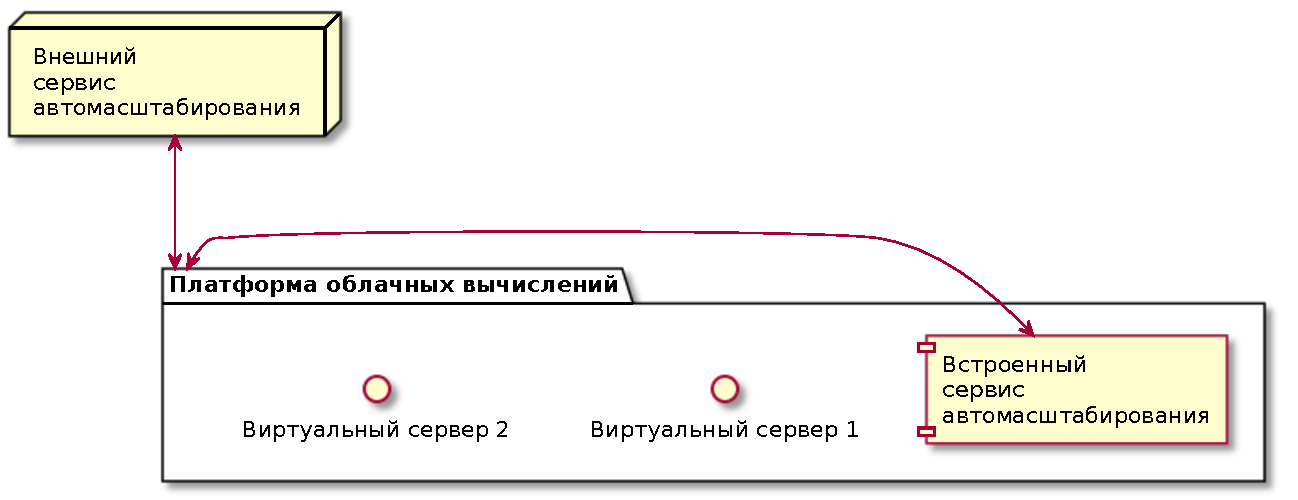
\includegraphics[width=\textwidth]{img/ext-int-scaler.pdf}
    \caption{Внешний и внутренний сервисы автомасштабирования}
    \label{ext-int-scaler}
\end{figure}

Причины появления таких сервисов могут быть разными, некоторые примеры приведены далее.
\begin{enumerate}
    \item Отсутствие решений автомасштабирования в используемой облачной платформе~\cite{fake-27}.
    \item Недостаточная эффективность встроенного сервиса автомасштабирования.
    
    Это может быть обусловлено спецификой конкретного приложения, которую встроенный сервис не учитывает, так как чаще всего они спроектированы без учёта специфики конкретных приложений.~\cite{fake-29}.
\end{enumerate}

На практике зачастую внешние сервисы автомасштабирования спроектированы и разработаны под одну конкретную платформу облачных вычислений~\cite{fake-30}.
При этом взаимодействие с другими платформами требует доработки реализации сервиса автомасштабирования как показано на рис.~\ref{ext-different-apis}. 
Это обусловлено значительной разницей в предоставляемых программных интерфейсах (API) разными платформами облачных вычислений~\cite{fake-31}.

\begin{figure}[hbtp]
    \centering
    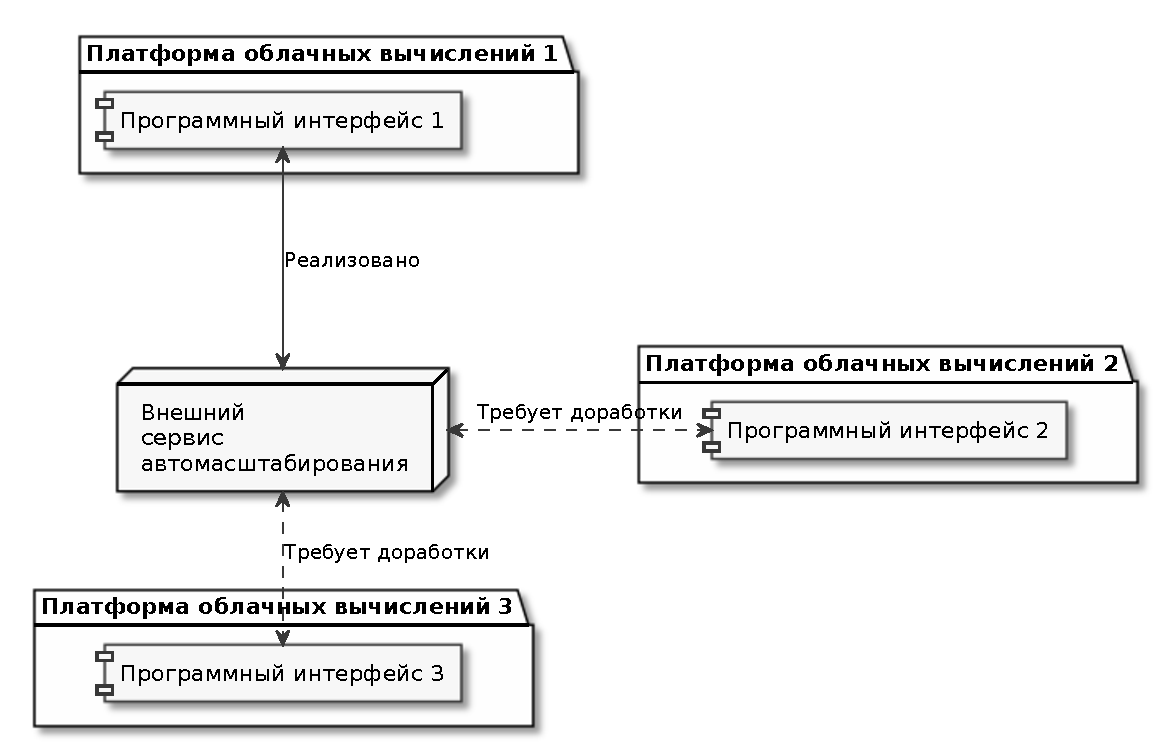
\includegraphics[width=\textwidth]{img/ext-different-apis.pdf}
    \caption{Проблема взаимодействия с разными платформами}
    \label{ext-different-apis}
\end{figure}
